\documentclass[11pt, titlepage]{article}
\usepackage{amsmath,amsthm,amssymb}
\usepackage{hyperref, pgf, tikz}
\usepackage{fancyhdr}
\usetikzlibrary{arrows}
\usepackage[margin=1.25in]{geometry}
\usepackage{graphicx}                     
\pagestyle{fancy}
\usepackage{array}
%\usepackage{wrapfig}

\lhead{Lab \#2}
\rhead{\thepage}
\cfoot{}

\title{Projectile Motion: The Ballistic Pendulum \\ \ \\ \large Lab \#2}
\author{Name: Avery Karlin \\ Partner: Alon Levin}
\date{}
\begin{document}

\maketitle

\begin{center}
\LARGE Projectile Motion: The Ballistic Penudulum
\end{center}

\section*{Objective}
The objective of the lab is to 
\section*{Introduction}

\section*{Procedures and Results}

\begin{figure}[p]
\centering
\hspace*{-10.5cm}
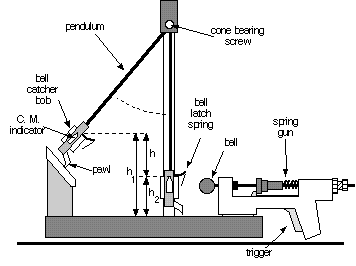
\includegraphics[scale=0.15, angle=270]{lab2.jpg}
\vspace*{19cm}
\end{figure}

\begin{center}
$$\text{Height of} h_2 \text{of pointer with pendulum catch in closest-to-average notch number} = $$
$$\text{Height of} h_1 \text{of pointer with pendulum freely suspended} = 0.055 m$$
$$h = h_2 - h_1 = $$
$$\text{Mass of ball m} = $$
$$\text{Mass of pendulum M (bob and support)} = $$
\begin{tabular}
{|m{7em}|m{7em}|}
\hline
Trials & Notch Number of Pendulum Catch \\
\hline
1 & \\
\hline
2 & \\
\hline
3 & \\
\hline
4 & \\
\hline
5 & \\\
\hline
Average & \\
\hline
\end{tabular}

$$\text{Vertical distance of fall, y} = $$
$$v_{x_o} \text{(calculated)} = $$
$$\text{Percent difference between results of part A and B} = $$
\begin{tabular}
{|m{7em}|m{7em}|}
\hline
Trials & Range\\
\hline
1 & \\
\hline
2 & \\
\hline
3 & \\
\hline
4 & \\
\hline
5 & \\\
\hline
Average & \\
\hline
\end{tabular}

\begin{tabular}
{|m{7em}|m{7em}|}
\hline
Angle of projection & Average range \\
\hline
$20^o$ & \\
\hline
$30^o$ & \\
\hline
$40^o$ & \\
\hline
$50^o$ & \\
\hline
$60^o$ & \\
\hline
$70^o$ & \\
\hline
\end{tabular}

\section*{Discussion}
Sample calculations for the non-measured data are as shown:

%Add more discussion here

\section*{Conclusion}


\end{document}
